
\documentclass[10pt,aps,prc,twocolumn]{revtex4-1}

\usepackage{tabularx} 
\usepackage{graphicx} 
\usepackage{hyperref}  
\usepackage{amssymb}  
\usepackage{amsmath}  
\usepackage[]{units}

\bibliographystyle{apsrev4-1}

\begin{document}
\title{Bias-Variance Trade-Off In Proton Radius Extractions From Electron Scattering Data} 
% a.k.a. How I Learned to Stop Worrying and Love the Bias

\author{Randall Evan McClellan}
\affiliation{Jefferson Lab, Newport News, VA 23606}
\author{Douglas Weadon Higinbotham}
\affiliation{Jefferson Lab, Newport News, VA 23606}
\author{Xuefei Yan}
\affiliation{Duke University, Durham, NC 27708}

\begin{abstract}
Intuitively, phenomenologists often assume that a more complex model will necessarily yield a more 
accurate discription of experimental data.   Herein we analyze this ansatz in the context of extracting 
the proton charge radius from simulatied charge form factor data.
We will show, due to the noise in the experimental data,
that a parsimonious extraction of the proton radius can in fact be the better model to use.
This result, which is contra to many previous papers that focused solely on bias,  provides a 
simple illustration the trade-off between bias and variance that is at the
heart of machine learning algorithms as well as the basis for regression regularization methods
where a biased model with a low variance can be the better predictive model then a low bias high
variance model.  
\end{abstract}

\maketitle

\section{Introduction}

The proton's charge radius, $r_p$, can be extracted
by determining the slope of the electric form factor as $Q^2$
approaches zero.   The relation between this slope and 
the radius is defined to be
$$
G_E(Q^2)
   =  1
   +  \sum_{n\ge 1} \frac{(-1)^n}{(2n+1)!}
      \left\langle r^{2n} \right\rangle \, Q^{2n} \>.
$$
Hence, $r_p$ can be determined from
$$
  r_p \equiv \sqrt{ \langle r^2 \rangle}
   = \left( -6  \left. \frac{\mathrm{d} G_E(Q^2)}{\mathrm{d}Q^2}
    \right|_{Q^{2}=0} \right)^{1/2} \>.
 $$
Of course, electron scattering cannot reach the exact $Q^2 = 0$ limit; thus,
an extrapolation is required to extract the charge radius from the experimental data.

In the recent literature, you can find a number of extractions of the proton radius ranging from
parsimonious fits of low Q$^2$ data~\cite{Griffioen:2015hta,Horbatsch:2016ilr,Higinbotham:2015rja} to 
extremely complex models with more than fifty free parameters~\cite{}.

A common criticism of the parsimonious models is the known prescence of bias. 
Proponents of the complex fits imply that bias must be avoided at any cost. 
In fact this was explicately stated in a classic Monte Carlo study where the 
presents of a bias was used to reject the then coming used parsimionous 
model~\cite{Borkowski:1975}.

We will show in this work that when building a statistical model, one needs to in fact 
consider both bias and variance.   Contrary to intuition, models with bias can in fact 
have better predictive power especially in cases where an extrapolation is required.

\section{Bias}

A very straight forward example of bias being used to rule out simpler models can be found in a Z. Physik
article from 1975~\cite{Borkowski:1975}; and while an older research article, its very strong conclusions are still 
noted to this day~\cite{Sick:2017aor} and a similar exercises have been done with other functions 
in Kruas~\textit{et al.}~\cite{Kraus:2014qua}.

As noted in~\cite{Hogg:2010yz}, the use of even an approximate generative model can be extremely important in understanding. 

The example problem, as presented in the Z. Physik paper, is extremely simple to reproduce.   
Randomly generate sets of faux change form factor faux in steps of $\unit[0.05]{fm^{-2}}$ from $\unit[0.1]{fm^{-2}}$ to 0.4, 0.8, 1.2,
and $\unit[1.6]{fm^{-2}}$ using the standard dipole function:
\begin{equation}
\label{sd}
\mathrm{G_D}(Q^2) = ( 1 + Q^2/(\unit[18.27]{fm^{-2}}))^{-2}.
\end{equation}
Perform fits on the resulting sets of faux data with linear and quadratic functions. The entire procedure is
then repeated many times to determine the mean of the extracted radii for each model. Table~\ref{ztable} reproduces the table found in the
Z. Physik article using python on a modern computer yielding only minor differences.
As the table clearly shows, the mean of $10^6$ linear fits is biased. 
Therefore, the authors conclude that the linear models should be rejected in favor of the lower-bias quadratic function.
They then proceed to extract the proton charge radius from real data using a five parameter fit: a quadratic charge form factor and three floating normalizations.

A Python notebook is included in the supplemental material.

\begin{table}
\label{ztable}
\caption{The following table shows the mean a$_0$ and radius terms from doing $10^6$ Monte Carlo simulations
for each range
where Eq.~\ref{sd} was used to generate faux data in $\unit[0.05]{fm^{-2}}$ steps with each points randomized using
0.5\% normal distribution.   The results clearly indicate that the linear fits are biased.   The input
radius was \unit[0.8113]{fm} (an a1/a0 term of $\unit[0.1097]{fm^{-1}}$) and an a0 of one.}
\begin{tabular}{c|cc|cc} \hline
interval       & \multicolumn{2}{c|}{linear fit} & \multicolumn{2}{c}{quadratic fit}  \\
fm$^{-2}$      & a$_0$      & radius          & a$_0$    & radius \\ \hline
 0.1 -- 0.4 & 1.000& 0.79& 1.000& 0.81 \\
 0.1 -- 0.8 & 0.999& 0.78& 1.000& 0.81 \\
 0.1 -- 1.2 & 0.997& 0.77& 1.000& 0.81 \\
 0.1 -- 1.6 & 0.996& 0.76& 1.000& 0.81 \\ \hline
\end{tabular}
\end{table}

\section{Variance}

While the mean of the results is indeed correct; when we run an experiment we typically do no get to run it $10^6$ times.
In particular in nuclear physics, the experiments are few and far between thus we need to carefully consider variance as
well as the bias when picking the statistical model to use.

If the authors of the Z. Phys. paper had decide to focus on variance instead of bias, they would have come to a very
different conclusion.

\begin{table}
\label{ztable}
\caption{The following table shows the variance of the a$_0$ and radius terms from doing $10^6$ Monte Carlo simulations
for each range
where Eq.~\ref{sd} was used to generate faux data in $\unit[0.05]{fm^{-2}}$ steps with each points randomized using
0.5\% normal distribution.   The results clearly indicate that the quadratic fits have a large variance.   The input
radius was \unit[0.8113]{fm} (an a1/a0 term of $\unit[0.1097]{fm^{-1}}$) and an a0 of one.}
\begin{tabular}{c|c|c} \hline
interval       & \multicolumn{1}{c|}{linear fit} & \multicolumn{1}{c}{quadratic fit}  \\
fm$^{-2}$   & sigma [fm]         &  sigma [fm] \\ \hline
 0.1 -- 0.4 & 0.0184&  0.1094 \\
 0.1 -- 0.8 & 0.0095&  0.0281 \\
 0.1 -- 1.2 & 0.0110&  0.0138 \\
 0.1 -- 1.6 & 0.0136&  0.0085 \\ \hline
\end{tabular}
\end{table}


Table~\ref{fulltable} shows more complete picture of the simulation results where the variance is shown along with the bias.
This table in fact shows nearly a textbook illustration of the trade-off between variance and bias with the simple fits
having a relatively high bias with a low variance while the quadratic fits have a low bias and high variance.

\begin{table*}
\label{fulltable}
\caption{The input radius was 0.8113 fm (an a1/a0 of $\unit[0.1097]{fm^{-1}}$).}
\begin{tabular}{cc|cccccc|cccccc} \hline
Data   & Range     & \multicolumn{6}{c|}{linear fit}                       & \multicolumn{6}{c}{quadratic fit}                    \\ 
Points & fm$^{-2}$ &   a0  & Radius&  a1/a0 &  Bias  & Sigma &  RMSE  &   a0  & Radius& a1/a0  &  Bias  & Sigma &  RMSE \\  \hline
7      & 0.1 -- 0.4 & 0.9995& 0.7948& -0.1053& -0.0044& 0.0184& 0.0189 & 1.0000& 0.8063& -0.1084& -0.0013& 0.1094& 0.1094\\
15     & 0.1 -- 0.8 & 0.9987& 0.7828& -0.1021& -0.0076& 0.0057& 0.0095 & 1.0000& 0.8096& -0.1092& -0.0005& 0.0281& 0.0281\\
22     & 0.1 -- 1.2 & 0.9975& 0.7712& -0.0991& -0.0106& 0.0030& 0.0110 & 0.9999& 0.8089& -0.1090& -0.0007& 0.0138& 0.0138\\
31     & 0.1 -- 1.6 & 0.9959& 0.7600& -0.0963& -0.0134& 0.0019& 0.0136 & 0.9998& 0.8075& -0.1087& -0.0010& 0.0085& 0.0085\\ \hline
\end{tabular}
\end{table*}

\begin{figure}[htbp]
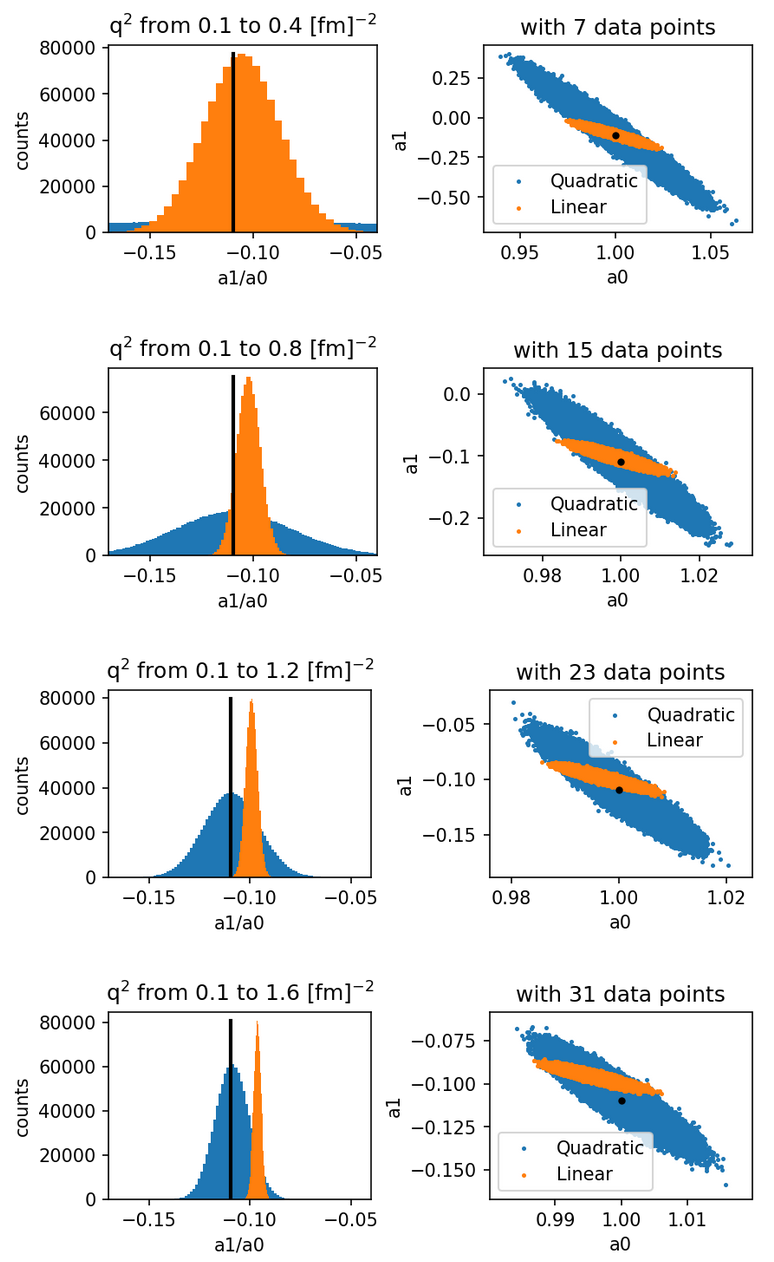
\includegraphics[width=\columnwidth]{Figure/zresult.png}
\caption{Bla bla bla.}
\end{figure}

\begin{table*}
\label{equaldatatable}
\caption{Same as before, but now with equal number of data points of each range.}
\begin{tabular}{cc|cccccc|cccccc} \hline
Data   & Range     & \multicolumn{6}{c|}{linear fit}                       & \multicolumn{6}{c}{quadratic fit}                    \\ 
Points & fm$^{-2}$ &   a0  & Radius&  a1/a0 &  Bias  & Sigma &  RMSE  &   a0  & Radius& a1/a0  &  Bias  & Sigma &  RMSE \\  \hline
31& 0.1 - 0.4 & 0.9995& 0.7951& -0.1054& -0.0043& 0.0098& 0.0107 & 1.0000& 0.8090& -0.1091& -0.0006& 0.0629& 0.0629 \\
31& 0.1 - 0.8 & 0.9987& 0.7829& -0.1021& -0.0076& 0.0041& 0.0086 & 1.0000& 0.8099& -0.1093& -0.0004& 0.0208& 0.0208  \\
31& 0.1 - 1.2 & 0.9974& 0.7712& -0.0991& -0.0106& 0.0026& 0.0109 & 0.9999& 0.8089& -0.1091& -0.0006& 0.0121& 0.0121  \\
31& 0.1 - 1.6 & 0.9959& 0.7600& -0.0963& -0.0134& 0.0019& 0.0136 & 0.9998& 0.8076& -0.1087& -0.0010& 0.0085& 0.0085  \\ 
\end{tabular}
\end{table*}


\section{Goldilocks Dilemma}

For any given statistical model, the goal is to find the optimal balance between bias and variance.   
In general, this can be written as:
\begin{equation}
\frac{d Bias^2 }{ d Complexity} = \frac{- d Variance }{ d Complexity }
\end{equation}

Thus going back to Table~\ref{fulltable} and checking the root mean square error, one can see that for the four ranges
one finds the 0.1 -- 0.8 range is actually optimal for the linear model and the 0.1 -- 1.6 range is optimal for the quadratic model. 
This is in complete contrast to the conclusion one draws when only considers bias as presented in Table~\ref{ztable}
though constant with the observation that the optimal specific form of the parameterization may depend on the $Q^2$ region
being fit~\cite{Alberico:2008sz}.
\begin{figure}
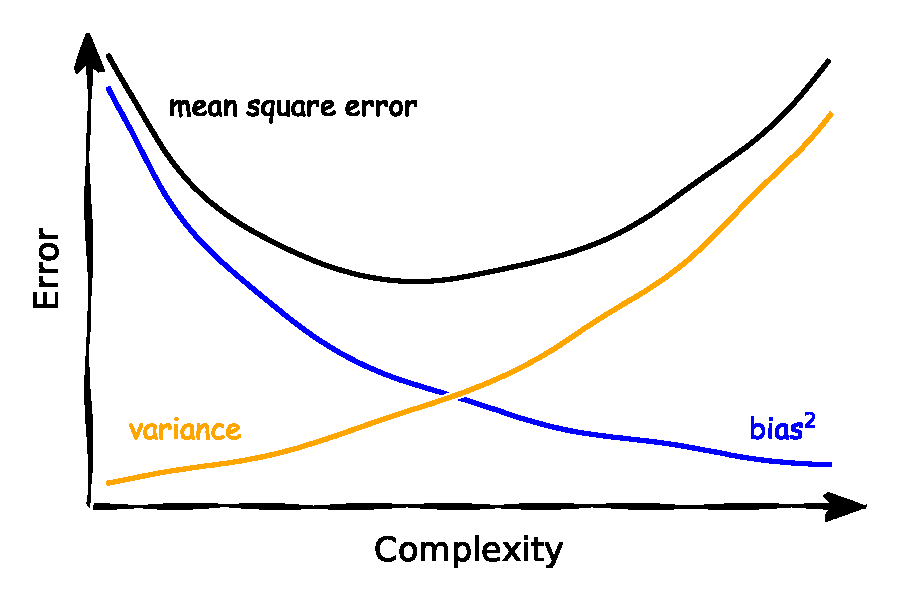
\includegraphics[width=\columnwidth]{Figure/biasvariance.pdf}
\caption{An illustration of the trade-off between bias and variance when selecting a statistical model.   Simple models
will have low variance but high bias (under-fitting) while complex models will have low bias but high variance (over-fitting).   
It is this trade-off that one seeks to balance.   While with repeated  Monte Carlo simulations it is trivial to find the optimal
predictive model for a give set of data; in the real world true model is typically unknown and one only gets preform a very limited number
of experiments and thus one relys on using real data and statistical methods for model selection~\cite{Hastie:2009}.
}
\end{figure}

It is interesting to repeat the Monte Carlo simulation for equal number of data points within each range
especially since, for any given experiment, the elastic scattering cross sections are significantly higher as lower values
of Q$^2$.

As shown in Table~\ref{equaldatatable}, the picture is even greyer as the root mean square error of the linear 
fit is nearly equal to the quadritic thus, assuming standard dipole was the true generating function,  experiments
with 31 data point and an uncertainty of 0.005 per point over a range of 0.1 to 0.8 and a different experiment
over a range of 0.1 to 1.6 would produce nearly idenitical if all other things were equal.

In this case, the choice of the parsimonious modeler to use the low Q$^2$ data would like be driven by the recugnition that as Q$^2$ increases
the extraction of a charge form factor is complicated by the growing influcance of the magnetic form factor while the use of the larger Q$^2$
range would likely be driven by a desire to form a more complet picture of the proton's structure (e.g. interest not only in the proton's radius
but also its higher order momentums).

\begin{equation}
\sigma / \sigma_{Mott} = eps G_E^2 + tau G_M^2
\end{equation}

\begin{figure}
\label{zoptimized}
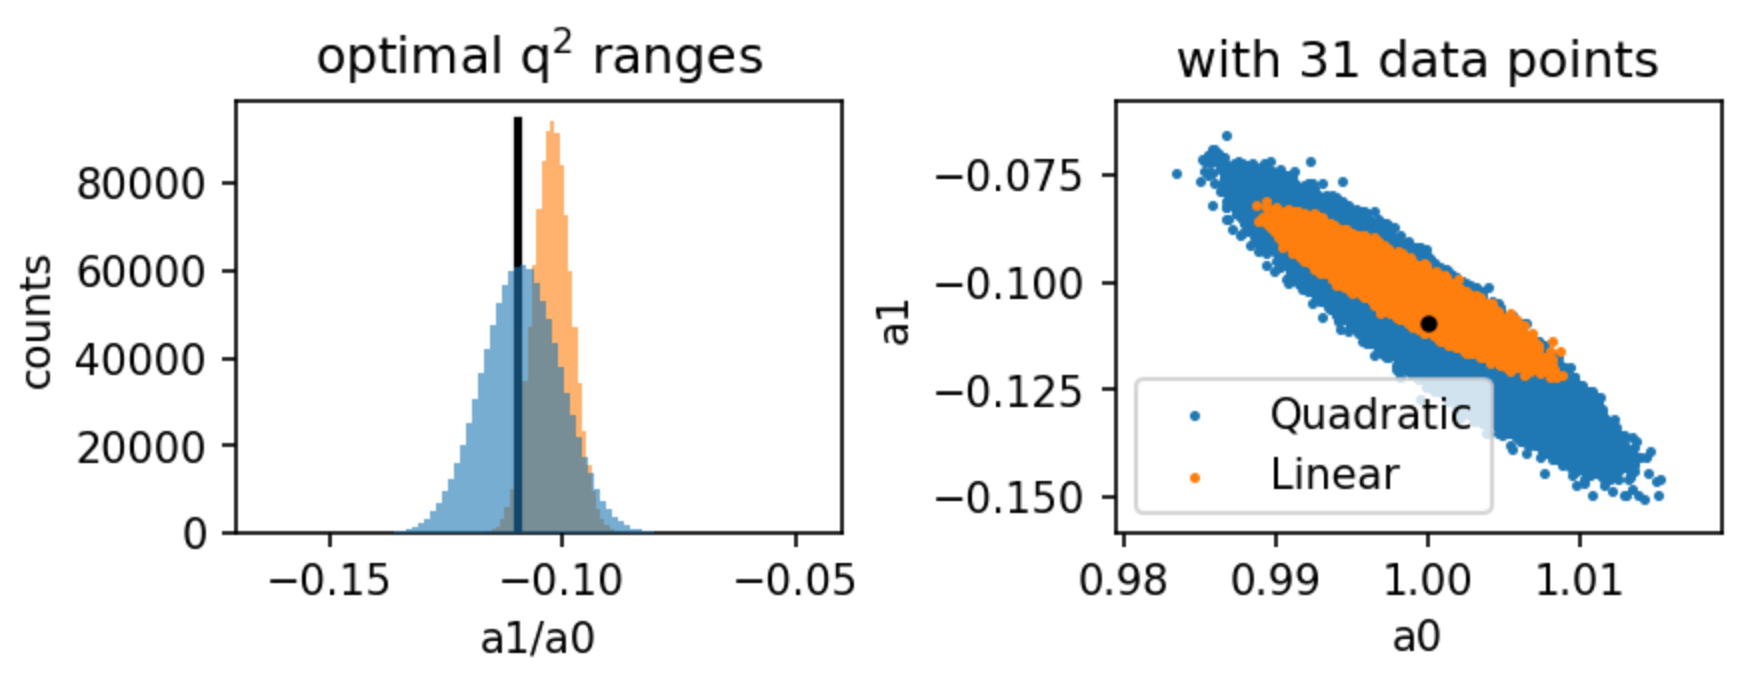
\includegraphics[width=\columnwidth]{Figure/zoptimized.png}
\caption{Shown is the result of million simulations and fits of linear fits  0.1 -- 0.8~fm$^{-2}$ 
and quadratic fits 0.1 -- 1.6~fm$^{-2}$ both with 31 eqaully spaced data points.    Using root mean
square error as the matrix, neither example is significantly better then the other for exacting the proton
radius   This is annaligous to a dart game between two eqaully skilled players though one who hits the bulls eye more 
often yet has a large spread (low bias but high variance) and another equally skilled player who has a tigher cluster of hits
but an offset (high bias but low variance).}
\end{figure}

The above illistration in fact suggests there are indeed two path forward for the modeler.   Either use simple models and extremely low Q2 
data or use more complex models that cover larger ranges of data.   It is worth noting that inorder to use larger ranges
of experimental data, one will need to model not only the charge form factor but also the exact details of  magnetic form factor
will start become quite important.


\section{Model Selection and the Modern Debate}

While this classic Monte Carlo example problem is over 40 years old, it actually points to exactly the split in the current electron
scattering proton radius extraction proceedures.     The parsimonious modelers who are focused solely on extracting a radius have
focused in on the low Q$^2$ region accepting accepting a higher level of bias in exchange for low variance while those modelers
who are interesting in extracting more information about the proton (i.e. higher order moments) fit longer Q$^2$ ranges and have
focused on complex models which while lower in bias come at a cost of higher varaince.  
And the end result has been an uncertainty on the electron scattering proton radius stuck at $\approx \unit[0.01]{fm}$ since 
L.~Hand~\textit{et al.} original fit in 1963~\cite{} as the increased complexity drives an increased variance.

Also, since we don't know the true model so one cannot exactly calculate the RMSE; so while exercises like this one are
extremely useful for making sets are models; in the end, the data must be used to select the approximate model. 
For this we relay on statistical modeling techinques such as chi2, reduced chi2, F-tests, A.I.C., B.I.C. to guide our selecton of
regression models and/or theoretical constraints.

In fact, statistics books warn about drawing too strong an inference from these types of Monte Carlos.   For example,
just because the linear model has a negative bias when compared to standard dipole, does not imply that it has a negative bias
to all possible models.
In fact, the Z.Physik paper itself rules out the very model it was using for model builting: i.e. drawing very strong conclusions from the standard dipole
function with its \unit[0.81]{fm} radius yet their five parameter fit (two charge form factor parameters and three normalization parameters)
gave a radius of \unit[0.87]{fm}.

Looking back to our example function, one can see that the range of the Saskatoon data (0.1 -- 0.8 fm$^{-2}$) could in fact be a reasonable
choice for extracting a radius and as shown much later if one redoes the Z.Physik fits but adopts the Saskatoon linear proceedure one finds
a radius of \unit[0.84]{fm}~\cite{Higinbotham:2015rja}.   Though want one really wants is a function with both low bias and low variance.

\section{Beyond Polynomial Expansions}

While one can cointue to increase the $Q^2$ range of the data, one will find that higher and higher order polynomials are required
to discribe the data and as shown in~\cite{Kraus:2014qua}, but this leads to ever increasing variance and instability as real data
isn't prefectly normally distriubuted as in these example Monte Carlo distributions.

To try to avoid these issues, one can impliment a bounded least squares fit based on a physical argument~\cite{Horbatsch:2016ilr} 
or try purely statastical appoaches such as machine learning regression such as stepwise regresson~\cite{Higinbotham:rja} 
to pick the appropriate order fit, though it would be far more statifying to simply find function that has 
both low bias and low varaince over a large range of $Q^2$.

While a Taylor series is the most general minimax function, it is not the only one.    If one explores (quote math book) one 
will find several other functions which are equally flexible yet have properties that may make them approxiate for the 
extrapolation problem at hand.   In particular, rational functions~\cite{Kelly:2004hm,PUckett:2017flj} 
and continued fractions~\cite{} have been shown to extrapolate well~\cite{}.

%The rational function or even a two parameter continued fraction 
%
%\begin{equation}
%G_E \simeq (a_0 + a_1 Q^2)/(1 + a_2 Q^2)
%\end{equation}
%
%We note that this deceptively simple form can be extended to give the correct asymmotic behiver
%as was done by J.J.~Kelly~\cite{Kelly:2004hm} and A.J.R.~Puckett {\it{et al.}}~\cite{Puckett:2017flj}.


\section{Summary}

The concept of a bias-varinace trade-off is key to regulariztion techniques such as stepwise regression, ridge regression and
statistical lasso.    By accepting some bias, these techniques tend to achieve a far superior mean square error then
the unregulated ordinary least squares solution of the same complexity.     

For the specific example of electron scattering, we have shown using the standard dipole function that 
the practice of simply concluding that a model with a higher predictive validity is truer is not valid 
assumption and that parsimonious modeling can in fact have the higher predictive validity depending on 
the exact range and precision of the data.

Further details of bias-variance trade-off are covered in detail in Shmueli's review article~\cite{Shmueli:2010}  
and as George Box was always known to say, "All models are wrong; but some are useful."

\bibliography{elastic}

\end{document}
